%% =============================================================================
%% main.tex -- Phase 1 project report in IEEE conference format.
%%
%% Derived from the official IEEE conference LaTeX template
%% (IEEE-conference-template-062824, "Template version as of 6/27/2024"),
%% linked from https://www.ieee.org/conferences/publishing/templates.html.
%%
%% Build (from inside report/):  ./sync_figures.sh && tectonic main.tex
%%
%% This file holds only the document structure (preamble, title, authors and
%% the order of sections). All prose lives in sections/*.tex, one file per
%% section, so that team members can edit different sections in parallel.
%% Every number in the text is read from the files in ../results/.
%% =============================================================================

% ---- Font encoding (must come before \documentclass) ------------------------
% IEEE papers are set in Times, which IEEEtran selects as the 8-bit font family
% "ptm". tectonic compiles with XeTeX, whose default Unicode encoding (TU) has
% no "ptm" font, so without this line the PDF silently falls back to Latin
% Modern. It is loaded before the class (\RequirePackage is the form of
% \usepackage allowed there) because IEEEtran measures its font while loading.
% With T1, tectonic (XeTeX) and Overleaf (pdfLaTeX) use the same Times fonts.
% Consequence: keep the .tex sources ASCII-only (write --, ``...'', $-110$).
\RequirePackage[T1]{fontenc}

\documentclass[conference]{IEEEtran}
% Conference mode disables \thanks; this re-enables it. The template uses the
% first-page footnote for funding; we use it for the course information.
\IEEEoverridecommandlockouts

% ---- Packages of the official template --------------------------------------
\usepackage{cite}                     % sorted, compressed citations: [1]--[3]
\usepackage{amsmath,amssymb,amsfonts} % display equations and math symbols
% The template also loads algorithmic.sty; the paper has no pseudocode, so it
% is not loaded (it would only add a harmless XeTeX encoding warning).
\usepackage{graphicx}                 % \includegraphics for the PDF figures
\usepackage{textcomp}                 % extra text symbols (kept from template)
\usepackage{xcolor}                   % color support (kept from template)

% ---- Packages added for this report -----------------------------------------
\usepackage{booktabs}                 % \toprule, \midrule, \bottomrule
\usepackage{url}                      % line-breakable \url{...}

% sync_figures.sh copies the figures from ../results/figures/ into figures/,
% so a figure is included by its file name, e.g. {feature_check.pdf}.
\graphicspath{{figures/}}

% Title and keywords are defined once and reused for the printed paper and for
% the PDF metadata below, so the two can never disagree.
\newcommand{\papertitle}{Indoor Positioning from Wi-Fi Fingerprints with
  Classical Machine Learning on UJIIndoorLoc (Phase~1)}
\newcommand{\paperkeywords}{Indoor positioning, Wi-Fi fingerprinting,
  UJIIndoorLoc, random forest, XGBoost, grouped cross-validation}

% hyperref must be loaded last because it redefines commands of other packages.
% hidelinks keeps references and citations clickable without colored boxes.
\usepackage[hidelinks]{hyperref}
\hypersetup{
  pdftitle    = {\papertitle},
  pdfauthor   = {Gauri Mehrotra, Ansh, Agnik Misra, Kartikey Gupta, Lokendra Singh},
  pdfsubject  = {Phase 1 report, Project 9: Indoor Location Prediction Using Wi-Fi Signals},
  pdfkeywords = {\paperkeywords},
}

% All five authors share one affiliation. It follows the template's author
% block (department / organization / city, country) and is defined once so
% that the five copies cannot drift apart.
\newcommand{\nstaffiliation}{%
  \textit{Newton School of Technology}\\
  \textit{Rishihood University}\\
  Sonipat, Haryana, India}

\begin{document}
% IEEEtran sets \flushbottom in two-column mode, which stretches the space
% between paragraphs when a float leaves a column a fraction of a line short.
% \raggedbottom lets a column end at its last full line instead.
\raggedbottom

\title{\papertitle%
  \thanks{Phase~1 report for Project~9, ``Indoor Location Prediction Using
  Wi-Fi Signals'', Team T084, Section~D. Code, data and results:
  {\urlstyle{tt}\url{https://github.com/Jitmisra/T084-wifi-indoor-positioning}}.}%
}

% Author order is the citation order (left to right, then the next row).
\author{%
  \IEEEauthorblockN{Gauri Mehrotra}
  \IEEEauthorblockA{\nstaffiliation\\
    Enrollment No.~2401010170\\
    gauri.mehrotra2024@nst.rishihood.edu.in}
  \and
  \IEEEauthorblockN{Ansh}
  \IEEEauthorblockA{\nstaffiliation\\
    Enrollment No.~2401010077\\
    ansh.2024@nst.rishihood.edu.in}
  \and
  \IEEEauthorblockN{Agnik Misra}
  \IEEEauthorblockA{\nstaffiliation\\
    Enrollment No.~2401010044\\
    agnik.misra2024@nst.rishihood.edu.in}
  % \and[<material>] puts <material> between two author blocks (default:
  % \hfill). Ending the paragraph here starts a second, centered row, which
  % gives a balanced 3 + 2 layout instead of an uneven automatic wrap.
  \and[\hfill\mbox{}\par\mbox{}\hfill]
  \IEEEauthorblockN{Kartikey Gupta}
  \IEEEauthorblockA{\nstaffiliation\\
    Enrollment No.~2401010214\\
    kartikey.2024@nst.rishihood.edu.in}
  \and
  \IEEEauthorblockN{Lokendra Singh}
  \IEEEauthorblockA{\nstaffiliation\\
    Enrollment No.~2401010254\\
    lokendra.singh2024@nst.rishihood.edu.in}
}

\maketitle

% IEEE rule: no citations, footnotes, math or special symbols in the abstract.
\begin{abstract}
% Abstract (included inside the abstract environment of main.tex, so no \section).
% IEEE rule: no citations, footnotes, math or special symbols, so "percent" is
% written out. Numbers: results/metrics/cv_check.csv (3.67 m random CV, 12.52 m
% test), feature_check.csv (15.87 -> 11.38 m), test_results.csv (Random Forest,
% XGBoost) and final_model.json (the final model).
GPS fails inside buildings, but the Wi-Fi signals a phone hears show where it
is. On the public UJIIndoorLoc data (three buildings, 520 access points), we
predict a scan's building, floor and position with classical machine learning.
Features, settings and the final model are chosen by user-group
cross-validation, which holds out whole users and their phones; the test set,
recorded months later mostly with new phones, is used once. Random
cross-validation would have promised our Baseline RF, a default random forest,
a mean 2D error of 3.67~m; on the test set it reached 12.52~m. Adding our AP-affinity features, which learn where each access
point is usually heard, cut its cross-validated error from 15.87~m to 11.38~m.
The final model, a tuned Random Forest, finds the building of every test scan
and the floor of 92.2 percent, with a mean 2D error of 7.42~m. No model is best
at every task (XGBoost finds more floors, 95.2 percent), and our three task
models share nothing, which motivates one multi-task network in Phase~2.

\end{abstract}

\begin{IEEEkeywords}
\paperkeywords.
\end{IEEEkeywords}

% ---- Main text (numbered sections I, II, ...) -------------------------------
% Section I: Introduction -- the problem, why it matters, the three tasks and
% our three contributions. Number: results/metrics/feature_check.csv
% (rssi+stats 15.87 m -> rssi+stats+affinity 11.38 m, user-group CV).
\section{Introduction}\label{sec:intro}

GPS works well outdoors, but inside buildings its signals are too weak to be
useful. Wi-Fi is a practical alternative: many buildings already have a Wi-Fi
network, so no new hardware is needed~\cite{he2016wifi}. A phone measures the
received signal strength (RSSI, in dBm) of every Wi-Fi access point (WAP) it
hears: $-30$~dBm is very strong and $-100$~dBm is barely heard. One
\emph{scan} lists these values, and this list works like a \emph{fingerprint}
of the place where it was taken. Fingerprinting records scans at known places
and locates a new scan by comparing it with
them~\cite{bahl2000radar,liu2007survey}. Indoor positioning can, for
example, guide a visitor to a room on a large campus.

We use the public UJIIndoorLoc dataset~\cite{torres2014ujiindoorloc} and solve
three tasks for every scan: predict its \emph{building} (one of three) and its
\emph{floor} (one of up to five), two classification tasks, and its
\emph{position} ($x$ and $y$ in meters), a regression task. The hard part is
testing fairly. Scans recorded in a row at one spot look almost the same, so a
random split rewards remembering scans instead of learning places. This is a
form of data leakage: information that would not be available in real use
reaches the model~\cite{kaufman2012leakage}. This report covers Phase~1,
classical machine learning; Phase~2 will build a multi-task neural network.
Our contributions are:
\begin{itemize}
\item \emph{A fair evaluation.} Features, settings and the final model are
  chosen by 5-fold user-group cross-validation (CV), which holds out whole
  users and their phones, and the test set is used only once. We also show
  how optimistic random CV is.
\item \emph{AP-affinity features}, our own idea. They learn from the training
  scans where each WAP is usually heard and describe a scan by the WAPs it
  hears. They cut the CV mean 2D error of a default random forest from 15.87 to
  11.38~m.
\item \emph{A tuned comparison} of kNN, Random Forest and XGBoost, with an
  error analysis that shows what Phase~2 must improve.
\end{itemize}

% Section II: Related Work -- fingerprinting with nearest neighbors, the
% dataset, tree models, neural networks on UJIIndoorLoc, leakage and grouped
% CV, and the gap. What each paper did or reported is taken from
% docs/literature_review.md and docs/literature_matrix.csv (source locations
% are given there). No result of our own appears in this section.
\section{Related Work}\label{sec:related}

\emph{Fingerprinting.} Surveys~\cite{liu2007survey,he2016wifi} cover the
field. The classic RADAR system~\cite{bahl2000radar} located a scan by the
recorded scans nearest to it in signal space, the nearest-neighbor
rule~\cite{cover1967nearest} behind kNN. Horus~\cite{youssef2005horus} modeled
the variation of the signals with probabilities. Both were tested on the
authors' own small testbeds (median error 2.94~m for RADAR, below 0.6~m on
average for Horus), so their errors cannot be compared with other studies.

\emph{The dataset.} UJIIndoorLoc~\cite{torres2014ujiindoorloc} was presented
as the first public Wi-Fi fingerprinting database with several buildings and
floors. Its validation file was recorded months after the training file,
partly by new users and phones, which makes it a realistic
test~\cite{torres2015comprehensive}. Torres-Sospedra
et~al.~\cite{torres2015comprehensive} compared many kNN settings on it, but
chose the best one on the file they report, so that result is optimistic.

\emph{Tree models.} A comparison of classifiers on UJIIndoorLoc found kNN the
most suitable, with boosting and bagging bringing a decision tree close to
it~\cite{bozkurt2015comparative}. We test two tree ensembles, random
forests~\cite{breiman2001random} and XGBoost~\cite{chen2016xgboost}, tuned and
with our own features.

\emph{Neural networks.} Nowicki and Wietrzykowski~\cite{nowicki2017loweffort}
classified building and floor on UJIIndoorLoc with a deep neural network. Kim
et~al.~\cite{kim2018scalable} trained one network with building, floor and
location outputs. CNNLoc~\cite{song2019cnnloc} used a convolutional neural
network, but its headline numbers are the best values of different runs, not
of one model.

\emph{Grouped CV.} For grouped data, random CV can seriously underestimate the
error, and grouped (block) CV is the better
choice~\cite{roberts2017crossvalidation}. UJIIndoorLoc shows this too: a
network that got building and floor right for 98.2\% of a random split of the
training file did so for only 91.1\% of the validation
file~\cite{nowicki2017loweffort}.

\emph{Gap.} We found no study that compares tuned kNN, random forests and
XGBoost on UJIIndoorLoc with every choice made by user-group CV and the
validation file used only once, as the test set. Phase~1 fills this gap. Our
models still predict building, floor and position separately; multi-task
learning~\cite{caruana1997multitask}, which learns related tasks together
through a shared representation, is the subject of Phase~2.

% Section III: Data and Exploratory Analysis. Numbers:
%   results/metrics/eda_summary.json (scans, users, phones, groups, dates,
%     WAPs, readings, 0.77 m per data meter, new phones),
%   results/metrics/cleaning.csv (76 / 634 / 508 removed, 18,719 left).
% "Mostly from one phone": 430 of the 508 scans with a reading of -30 dBm or
% stronger come from phone 19 (count with indoorloc.data on trainingData.csv).
\section{Data and Exploratory Analysis}\label{sec:data}

\begin{figure}[t]
  \centering
  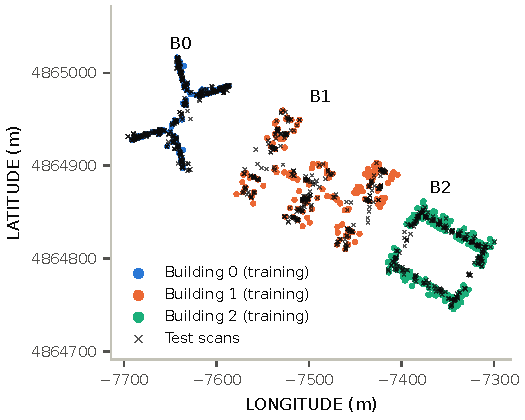
\includegraphics[width=0.9\columnwidth]{eda_campus_map.pdf}
  \caption{Where the scans were taken: training positions colored by building
  and test scans as crosses (Web-Mercator meters). Most test scans lie close
  to training positions.}
  \label{fig:campus}
\end{figure}

UJIIndoorLoc~\cite{torres2014ujiindoorloc} is dataset~310 of the UCI Machine
Learning Repository, recorded with smartphones in three buildings of
Universitat Jaume~I in Spain (Fig.~\ref{fig:campus}). Buildings~0 and~1 have
four floors and building~2 has five: 13 building--floor classes. Each row is
one scan: the RSSI of 520 WAPs, the building, floor and position, and the user
and phone ids. Positions are Web-Mercator meters; one such meter is about
0.77~m on the ground, and we report all errors in these dataset meters.

We train on the file \texttt{trainingData.csv}: 19,937 scans recorded from
30~May to 20~June 2013 by 18 users with 16 phones. Our \emph{test set} is the
UCI file \texttt{validationData.csv}: 1,111 scans recorded from 19~September to
8~October 2013 with 11 phones. It is hard for three reasons: it was recorded
about three months after the last training scan; 9 of its 11 phones never
appear in training, and they took 64.3\% of the test scans; and 55 of the WAPs
it hears are never heard in training, so no model can use them.

A scan hears only a few WAPs (17.82 on average in the cleaned training data,
16.48 in the test set), so 96.6\% of the training readings are ``not heard''.
The files store ``not heard'' as $+100$, which would look like the strongest
possible signal. We replace it by $-110$~dBm in both files: weaker than the
weakest real reading ($-104$~dBm), so ``not heard'' means ``very weak''.

We clean only the training file; the test file is used exactly as published.
In this order, we drop scans that hear no WAP (76), exact duplicate rows (634)
and scans with any reading of $-30$~dBm or stronger (508), which are
implausibly strong and come mostly from one phone. This leaves 18,719 training
scans. We keep only the 464 WAP columns heard in the cleaned training data,
because a WAP that is never heard tells a model nothing. Users who shared a
phone form one group, so the 18 training users form 16 user--device groups,
which we use for a fair split (Section~\ref{sec:method}).

% Section IV: Method -- fair evaluation, features (with AP-affinity), models,
% tuning, the final-model rule and the metrics. Settings and grids:
% src/indoorloc/config.py; chosen settings: results/tuning/best_params.json.
% The example weights (0.27, 0.05, almost 0) and r_min = -105 dBm come from
% indoorloc.features.APAffinity fitted on the cleaned training data.
\section{Method}\label{sec:method}

\subsection{Fair Evaluation}\label{sec:fair}
Because a person records several scans in a row at one spot with one phone,
random CV almost always leaves training scans from the same spot, person and
phone for a held-out scan. We therefore use 5-fold \emph{user-group
cross-validation (CV)}~\cite{roberts2017crossvalidation}, the GroupKFold of
scikit-learn~\cite{pedregosa2011scikit} with the 16 user--device groups: each
fold holds out whole groups, so every model is tested on people and phones
that it has not seen, as for most of the test set (9 of its 11 phones are
new). Every choice (features, settings,
final model) is made with these folds on the training data only, and all that
a model learns from data, including the kept WAP columns and the AP-affinity
profiles, is learned again in each fold. The test set is used once, at the
very end: each model is fitted on all 18,719 training scans and predicts the
1,111 test scans. For comparison only, we also score the Baseline RF with
\emph{random CV} (shuffled 5-fold).

\subsection{Features}\label{sec:features}
We compare three feature sets: \emph{rssi}, the RSSI of the kept WAPs (464
columns on the full training data); \emph{rssi+stats}, which adds three
\emph{signal statistics} (the number of WAPs heard, the strongest reading and
the mean of the heard readings); and \emph{rssi+stats+affinity}, which adds our
eight \emph{AP-affinity} columns.

AP-affinity starts from a simple idea: if a phone hears a WAP that is mostly
heard in building~1 on floor~2, the phone is probably there too. It is learned
from the training rows only, in two steps. First, every WAP heard in at least
five training scans gets a \emph{profile}: the share of its scans in each
building (3 values), its mean floor and its mean position (2 values), each a
weighted mean over the training scans that hear it. A stronger reading usually
means that the phone was closer to the WAP, so it gets a larger weight
\begin{equation}
  w(r)=\left(\frac{r-r_{\min}}{-r_{\min}}\right)^{e},
  \label{eq:weight}
\end{equation}
where $r$ is the reading in dBm, $r_{\min}$ is 1~dB below the weakest training
reading ($-105$~dBm on the full training data), $e\approx2.718$, and $w=0$ if
the WAP is not heard. This ``powed'' formula~\cite{torres2015comprehensive}
gives $w=0.27$ at $-40$~dBm, $0.05$ at $-70$~dBm and almost 0 at $-100$~dBm.
Second, a scan $s$ is described by the weighted average of the profiles of the
known WAPs that it hears:
\begin{equation}
  \mathbf{p}_j=\frac{\sum_i w_{ij}\,\mathbf{t}_i}{\sum_i w_{ij}},\qquad
  \mathbf{a}(s)=\frac{\sum_j w_{sj}\,\mathbf{p}_j}{\sum_j w_{sj}},
  \label{eq:affinity}
\end{equation}
where $\mathbf{p}_j$ is the profile of WAP~$j$, $w_{ij}$ the weight of WAP~$j$
in scan~$i$, and $\mathbf{t}_i$ holds the targets of training scan~$i$ (three
0/1 building indicators, floor, $x$, $y$). The 6 values of $\mathbf{a}(s)$ and
the position of the strongest known WAP in the scan give 8 columns; a scan
that hears no known WAP gets the training means.

\emph{Missing values and scaling.} A WAP that is not heard gets $-110$~dBm in
both files, below every real reading. We add no separate heard/not-heard
column per WAP: for a tree, a split below $-105$~dBm already means ``not
heard'', and \texttt{n\_heard} counts the heard WAPs. We do not scale the RSSI:
trees use only the order of the values, and all RSSI columns share one unit
(dBm), so kNN treats them alike. Nothing is ever fitted on the test set.
Scaling, fitted on the training data only, is needed in Phase~2, since neural
networks train badly on unscaled inputs.

\subsection{Models}\label{sec:models}
Each method predicts building, floor and position with three separate models,
one per task: two classifiers and one regressor with two outputs ($x$, $y$),
built with scikit-learn~\cite{pedregosa2011scikit} and the XGBoost
library~\cite{chen2016xgboost}.
\begin{itemize}
\item \emph{Baseline RF}: a random forest~\cite{breiman2001random} with 300
  trees and default settings on rssi+stats.
\item \emph{kNN}~\cite{cover1967nearest} on rssi: the vote (building, floor)
  or mean position of the $k$ training scans with the closest RSSI values,
  plain or weighted by closeness.
\item \emph{Random Forest} on rssi+stats+affinity: 300 trees, each trained on
  a random sample of the scans with a random subset of the features tried at
  each split; the trees vote or average~\cite{breiman2001random}.
\item \emph{XGBoost} on rssi+stats+affinity: trees added one at a time, each
  correcting the errors of those before it~\cite{chen2016xgboost}; learning
  rate (0.1), row sample (0.85) and column sample (0.5) are fixed.
\end{itemize}
In formulas: kNN compares two scans $\mathbf{r},\mathbf{r}'$ (RSSI vectors)
with the Euclidean or the Manhattan distance,
\begin{equation}
  d_2=\sqrt{\textstyle\sum_j (r_j-r'_j)^2},\qquad
  d_1=\textstyle\sum_j |r_j-r'_j|.
  \label{eq:knn}
\end{equation}
A classification tree picks, at each node, the split that most lowers the Gini
impurity $G=1-\sum_c p_c^2$, where $p_c$ is the share of class $c$ in the node
($G=0$ when the node is pure); a regression tree lowers the squared error.
XGBoost builds its prediction step by step,
\begin{equation}
  F_m(\mathbf{x})=F_{m-1}(\mathbf{x})+\eta\,f_m(\mathbf{x}),
  \label{eq:boost}
\end{equation}
where each new tree $f_m$ is fitted to reduce the remaining loss and
$\eta=0.1$ is the learning rate.

\begin{table}[t]
  \caption{Tuned Settings: Values Tried and the Value Chosen by CV for Each
  Task (B: Building, F: Floor, P: Position)}
  \label{tab:grids}
  \centering
  \footnotesize
  \setlength{\tabcolsep}{4pt}
  \begin{tabular}{@{}llccc@{}}
    \toprule
    Setting & Values tried & B & F & P \\
    \midrule
    \multicolumn{5}{@{}l}{\emph{kNN} (28 settings)} \\
    n\_neighbors ($k$) & 1, 3, 5, 7, 9, 11, 15 & 1 & 5 & 3 \\
    weights & uniform, distance & unif. & unif. & dist. \\
    metric & Euclidean, Manhattan & Eucl. & Manh. & Eucl. \\
    \midrule
    \multicolumn{5}{@{}l}{\emph{Random Forest} (300 trees, 6 settings)} \\
    max\_features & sqrt, 0.2, 0.5 & sqrt & 0.5 & 0.5 \\
    min\_samples\_leaf & 1, 4 & 1 & 4 & 1 \\
    \midrule
    \multicolumn{5}{@{}l}{\emph{XGBoost} (6 settings)} \\
    max\_depth & 4, 6, 10 & 4 & 4 & 10 \\
    n\_estimators & 300, 600 & 300 & 300 & 600 \\
    \bottomrule
  \end{tabular}
\end{table}

\subsection{Tuning and the Final Model}\label{sec:tuning}
Each model has a small grid (Table~\ref{tab:grids}), and every setting is
scored on the same five folds. Because each task has its own model, each task
picks its own best setting: the highest CV accuracy for building and floor, the
lowest CV mean 2D error for position. Before using the test set, we fixed the
rule for the final model: the tuned model (kNN, Random Forest or XGBoost) with
the lowest CV mean 2D error.

\subsection{Metrics}\label{sec:metrics}
Building and floor accuracy are the shares of scans with the right building
and floor. For the position we report the mean absolute error (MAE) in $x$ and
$y$ and the mean and median \emph{2D error}, the straight-line distance between
the predicted and the true position: for test scan $i$ with true position
$(x_i,y_i)$ and prediction $(\hat x_i,\hat y_i)$,
\begin{equation}
  \mathrm{MAE}_x=\tfrac{1}{N}\textstyle\sum_i|\hat x_i-x_i|,\quad
  e_i=\sqrt{(\hat x_i-x_i)^2+(\hat y_i-y_i)^2}.
  \label{eq:metrics}
\end{equation}
To see where the error comes from, we
split the test scans into three cases (building wrong; building right but floor
wrong; both right) and give each case's share of scans, mean 2D error and share
of the total error. We also compare test scans from seen and new phones.

% Section V: Results. Numbers (all under results/metrics/):
%   feature_check.csv (Fig. feature check), cv_check.csv (Table cvcheck),
%   cv_results.csv and final_model.json (CV errors, final model),
%   test_results.csv (Table test), error_breakdown.csv (Table breakdown),
%   floor_confusion.csv (Fig. confusion; 81 of the 87 wrong floors are one
%   floor off), per_phone.csv (seen and new phones, last paragraph).
\section{Results}\label{sec:results}

\begin{figure}[t]
  \centering
  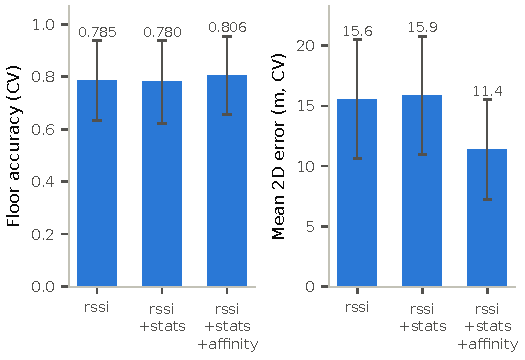
\includegraphics[width=0.95\columnwidth]{feature_check.pdf}
  \caption{Feature check: the Baseline RF settings on the three feature sets
  under user-group CV (bars: mean over the five folds; error bars: standard
  deviation). Floor accuracy is shown as a fraction.}
  \label{fig:features}
\end{figure}

\subsection{Feature Check}\label{sec:res-features}
Fig.~\ref{fig:features} shows the Baseline RF settings on the three feature
sets under user-group CV. The signal statistics did not help: the mean 2D error
rose slightly from 15.55 to 15.87~m and floor accuracy fell from 78.5\% to
78.0\%. AP-affinity helped clearly: the error fell to 11.38~m and floor accuracy
rose to 80.6\%. We keep the statistics in the full set because the three sets
are nested and the full set scored best; we did not test rssi plus AP-affinity
alone. The wide error bars show that the folds differ a lot, as each holds out
different people and places.

\begin{table}[t]
  \caption{The Baseline RF Scored in Three Ways}
  \label{tab:cvcheck}
  \centering
  \footnotesize
  \begin{tabular}{@{}lrrr@{}}
    \toprule
    Evaluation & Building (\%) & Floor (\%) & Mean 2D error (m) \\
    \midrule
    Random CV     & 100.0 & 99.9 &  3.67 \\
    User-group CV &  99.7 & 78.0 & 15.87 \\
    Test set      &  99.8 & 91.2 & 12.52 \\
    \bottomrule
  \end{tabular}
\end{table}

\subsection{Random CV Is Too Optimistic}\label{sec:res-cv}
For the same Baseline RF, random CV promised 99.9\% floor accuracy and a mean
2D error of 3.67~m, but the test set gave 91.2\% and 12.52~m
(Table~\ref{tab:cvcheck}): random CV tests the model on scans that look
almost like its training scans (same spot, person and phone). User-group CV
(15.87~m) is even stricter than the test set, as a held-out user may be the
only one who recorded some places. It errs on the safe side and needs no test data, so we
make all choices with it.

\begin{figure*}[t]
  \centering
  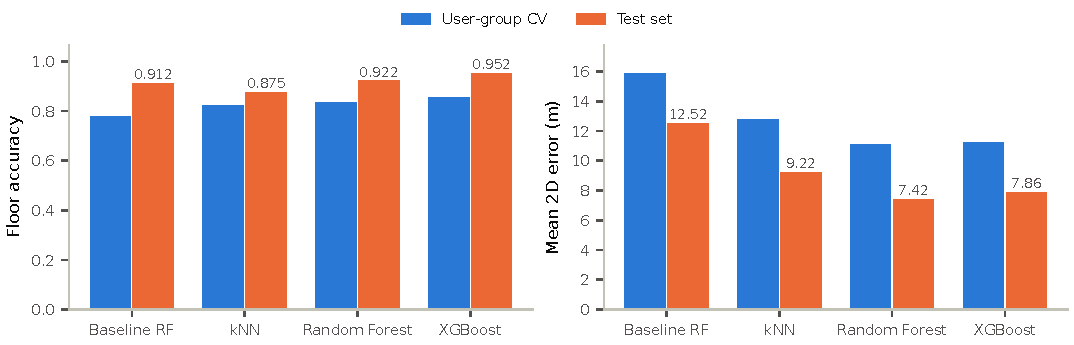
\includegraphics[width=0.9\textwidth]{model_comparison.pdf}
  \caption{Floor accuracy (as a fraction) and mean 2D error of the four models
  in user-group CV and on the test set (test values above the bars).}
  \label{fig:models}
\end{figure*}

\begin{table}[t]
  \caption{Results on the Test Set (1,111 Scans)}
  \label{tab:test}
  \centering
  \footnotesize
  \setlength{\tabcolsep}{3.5pt}
  \begin{tabular}{@{}lrrrrrr@{}}
    \toprule
    & Bldg. & Floor & MAE $x$ & MAE $y$ & \multicolumn{2}{c}{2D error (m)} \\
    \cmidrule(l){6-7}
    Model & (\%) & (\%) & (m) & (m) & Mean & Median \\
    \midrule
    Baseline RF   &  99.8 & 91.2 & 8.68 & 7.40 & 12.52 & 7.70 \\
    kNN           &  99.8 & 87.5 & 6.12 & 5.70 &  9.22 & 5.88 \\
    Random Forest & \textbf{100.0} & 92.2 & \textbf{4.77} & \textbf{4.64}
                  & \textbf{7.42} & \textbf{5.34} \\
    XGBoost       & \textbf{100.0} & \textbf{95.2} & 5.18 & 4.77 & 7.86 & 6.19 \\
    \bottomrule
  \end{tabular}
\end{table}

\subsection{Model Comparison}\label{sec:res-models}
Random Forest had the lowest CV mean 2D error (11.09~m, against 11.25~m for
XGBoost and 12.75~m for kNN), so by our rule it is the final model. On the test
set (Table~\ref{tab:test}) it found the building of every scan and the floor of
92.2\%, with a mean 2D error of 7.42~m, against 12.52~m for the Baseline RF.
The four models keep the same order by mean 2D error in CV and on the test set
(Fig.~\ref{fig:models}), so the choice made with CV holds. XGBoost, however,
found the most floors (95.2\% on the test set, 85.4\% in CV): no model is best
at every task.

\begin{table}[t]
  \caption{Where the Test Error Comes From}
  \label{tab:breakdown}
  \centering
  \footnotesize
  \setlength{\tabcolsep}{4pt}
  \begin{tabular}{@{}lrrr@{}}
    \toprule
    & Share of & Mean 2D & Share of total \\
    Case & scans (\%) & error (m) & error (\%) \\
    \midrule
    \multicolumn{4}{@{}l}{\emph{Random Forest}} \\
    Building wrong              &  0.0 &    -- &  0.0 \\
    Building right, floor wrong &  7.8 & 13.06 & 13.8 \\
    Both right                  & 92.2 &  6.94 & 86.2 \\
    \midrule
    \multicolumn{4}{@{}l}{\emph{XGBoost}} \\
    Building wrong              &  0.0 &    -- &  0.0 \\
    Building right, floor wrong &  4.8 & 14.78 &  9.0 \\
    Both right                  & 95.2 &  7.52 & 91.0 \\
    \bottomrule
  \end{tabular}
\end{table}

\begin{figure*}[t]
  \centering
  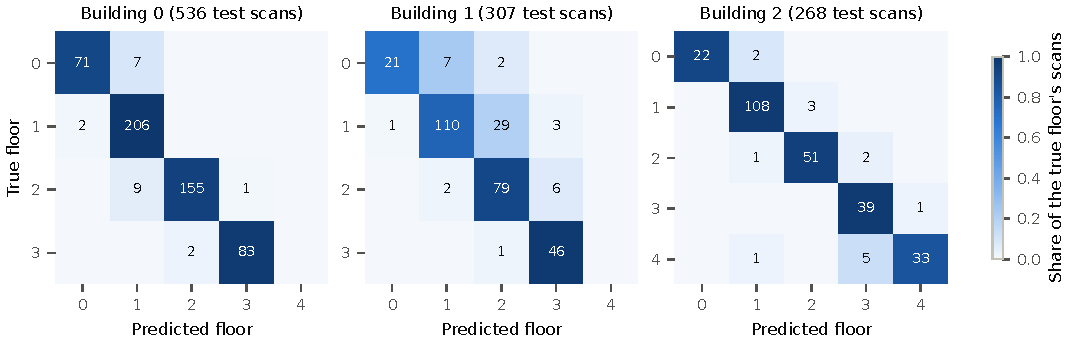
\includegraphics[width=0.95\textwidth]{floor_confusion.pdf}
  \caption{Floor confusion of the final model (Random Forest) on the test set:
  test scans per true and predicted floor; colors show the true floor's share.}
  \label{fig:confusion}
\end{figure*}

\subsection{Where the Error Comes From}\label{sec:res-errors}
Neither Random Forest nor XGBoost put a test scan in the wrong building; the
Baseline RF and kNN did so twice each. For the Random Forest, 87 scans (7.8\%) have the
right building but the wrong floor, and their mean 2D error (13.06~m) is nearly
twice that of the scans with both right (6.94~m; Table~\ref{tab:breakdown}).
Still, 86.2\% of the total error comes from the scans with both right: the main
remaining problem is the position within the right floor. Of the 87 floor
mistakes, 81 are one floor up or down (Fig.~\ref{fig:confusion}), and
building~1 has the most; for example, 29 of its floor-1 scans were placed on
floor~2. XGBoost makes fewer floor mistakes (53) but has a higher error when
both are right (7.52~m).

New phones are harder. On the 397 test scans from the 2 phones seen in
training, the Random Forest has a mean 2D error of 5.84~m and a floor accuracy
of 93.7\%; on the 714 scans from the 9 new phones, 8.30~m and 91.3\%. All four
models are worse on new phones.

% Section VI: Phase 2 Gap and Conclusion. Numbers: results/metrics/
% test_results.csv, feature_check.csv, error_breakdown.csv, per_phone.csv and
% cv_check.csv (all repeated from Section V).
\section{Phase 2 Gap and Conclusion}\label{sec:conclusion}

\emph{The gap.} Our three task models are separate and share nothing, and the
results point to what this misses. First, no model is best at every task:
XGBoost finds the most floors (95.2\%), Random Forest the best positions
(7.42~m). Second, AP-affinity, a
hand-made way of sharing location knowledge (where each WAP is heard) with all
three tasks, gave our largest gain (CV error from 15.87 to 11.38~m); a model
that learns such shared knowledge by itself may gain more. Third, most of the
remaining error is position error on the right floor (86.2\% of the Random
Forest's total error), and new phones are harder than seen ones (8.30~m
against 5.84~m).

\emph{Phase~2} will train one multi-task neural
network~\cite{caruana1997multitask} that learns building, floor and position
together: shared layers used by all three tasks, then three output heads. Kim
et~al.~\cite{kim2018scalable} showed that one network with building, floor and
location outputs can be trained on UJIIndoorLoc. We will evaluate our network
with the same user-group CV, test set and metrics, and compare it with our
Phase~1 models.

\emph{Conclusion.} Fair testing matters most: random CV promised 3.67~m, but
the Baseline RF reached 12.52~m on the test set. Chosen by user-group CV, the
final Random Forest with AP-affinity found every building and 92.2\% of the
floors, with a mean 2D error of 7.42~m.


% ---- Back matter ------------------------------------------------------------
% Unnumbered, course-specific section placed before the references.
% Unnumbered back-matter section; keep the roles consistent with README.md.
\section*{Team Contributions}
Gauri Mehrotra: problem and literature review. Ansh: data quality, EDA and the
fair split. Agnik Misra: features (signal statistics and AP-affinity). Kartikey
Gupta: models, tuning and results. Lokendra Singh: error analysis and the
Phase~2 gap.


% IEEE reference style. IEEEtran.bst ships with every TeX distribution and with
% Overleaf; references.bib holds only the works cited in the text.
% \IEEEtriggeratref{n} starts a new column at reference n, which balances the
% two columns of the last page (IEEEtran HOWTO). 14 fits the current layout;
% re-check the last page after any edit.
\IEEEtriggeratref{14}
\bibliographystyle{IEEEtran}
\bibliography{references}

\end{document}
